\begin{figure}[!htbp]
	\centering
	\begin{subfigure}{0.4\textwidth}
	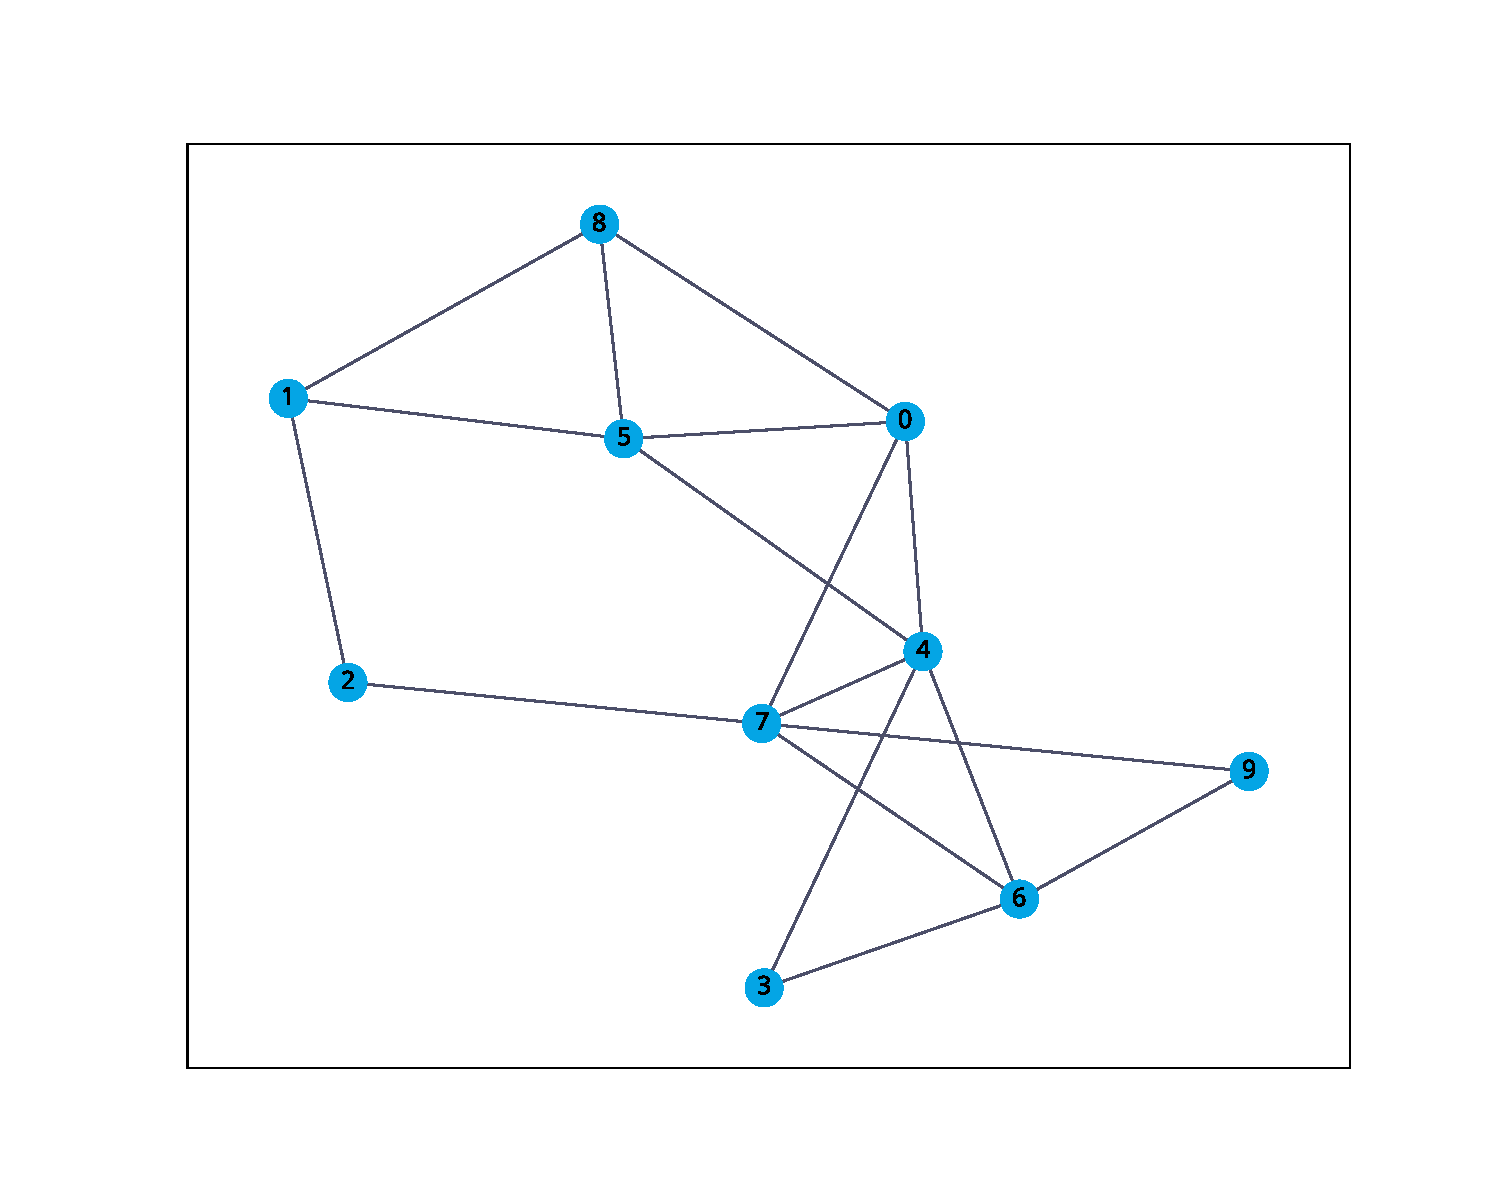
\includegraphics[width=\textwidth]{pictures/plots/10.pdf}
	\caption{\scriptsize$\abs{V} = 10$ nodes and $\abs{E} = 22$ links. (Small)}
	\end{subfigure}
	\quad
	\begin{subfigure}{0.4\textwidth}
	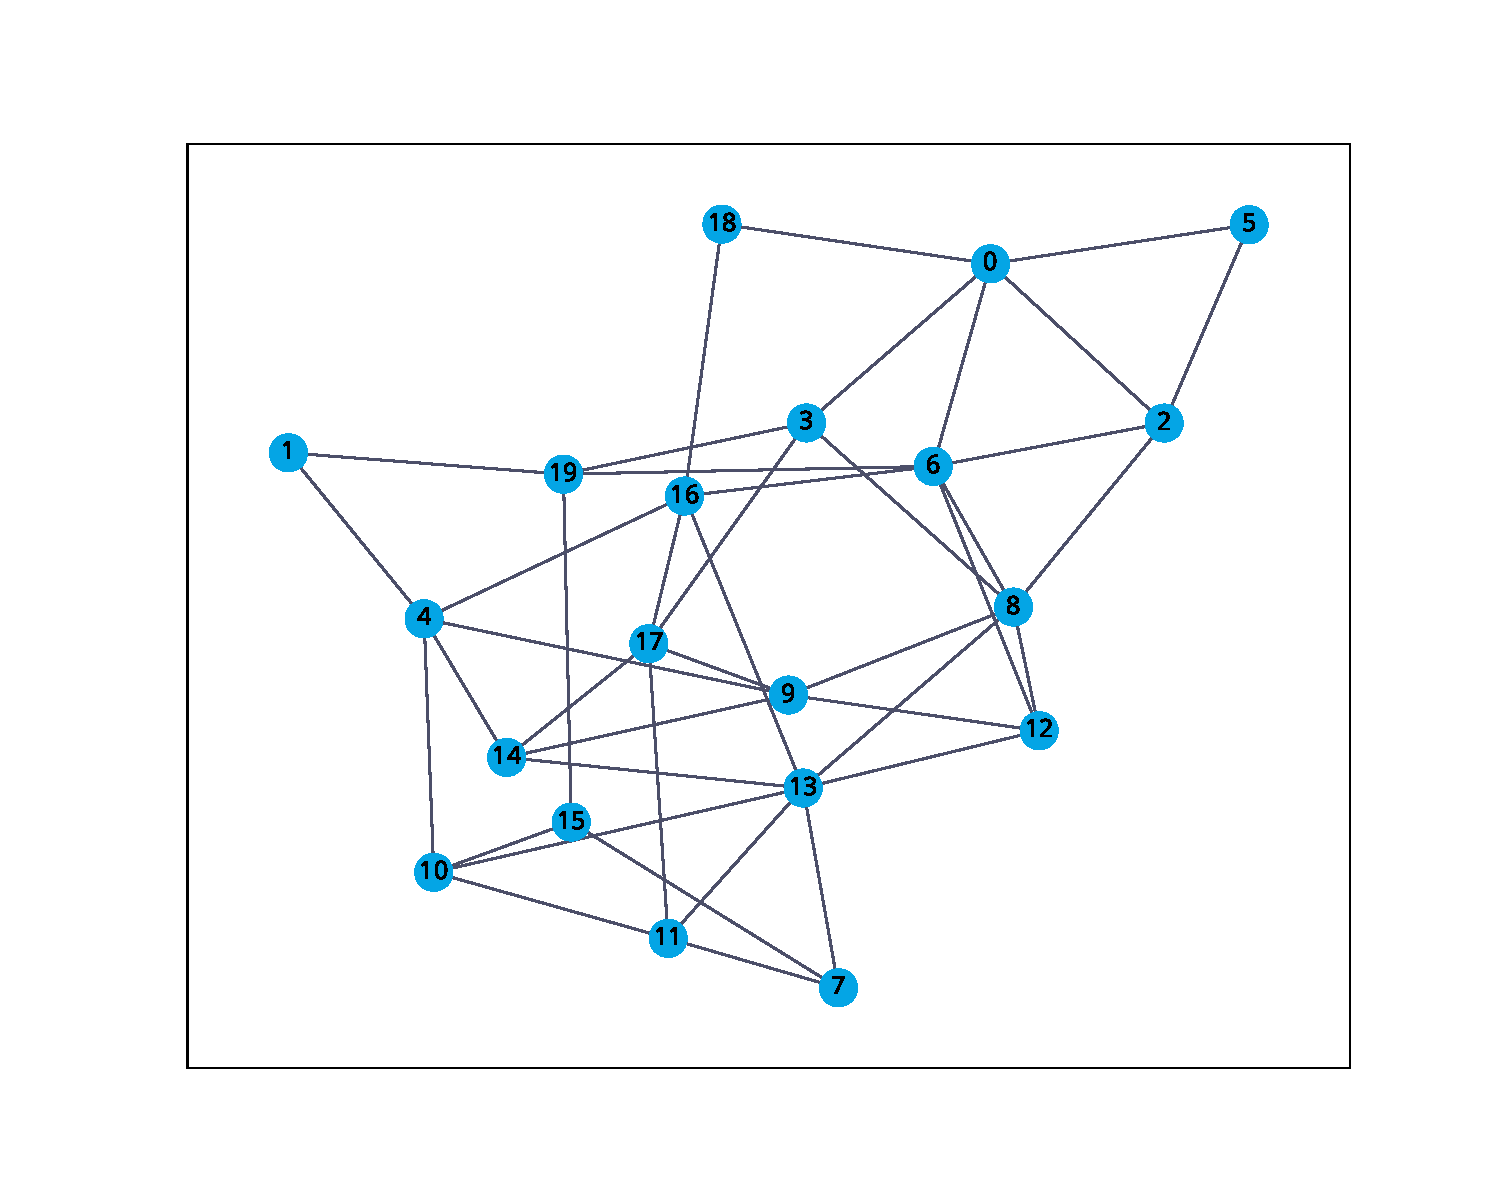
\includegraphics[width=\textwidth]{pictures/plots/20.pdf}
	\caption{\scriptsize$\abs{V} = 20$ nodes and $\abs{E} = 42$ links. (Large)}
	\end{subfigure}
	\label{fig:toynetworks}
\end{figure}
%
% \begin{figure}[!htbp]
% 	\centering
% 	\begin{subfigure}{0.49\textwidth}
% 	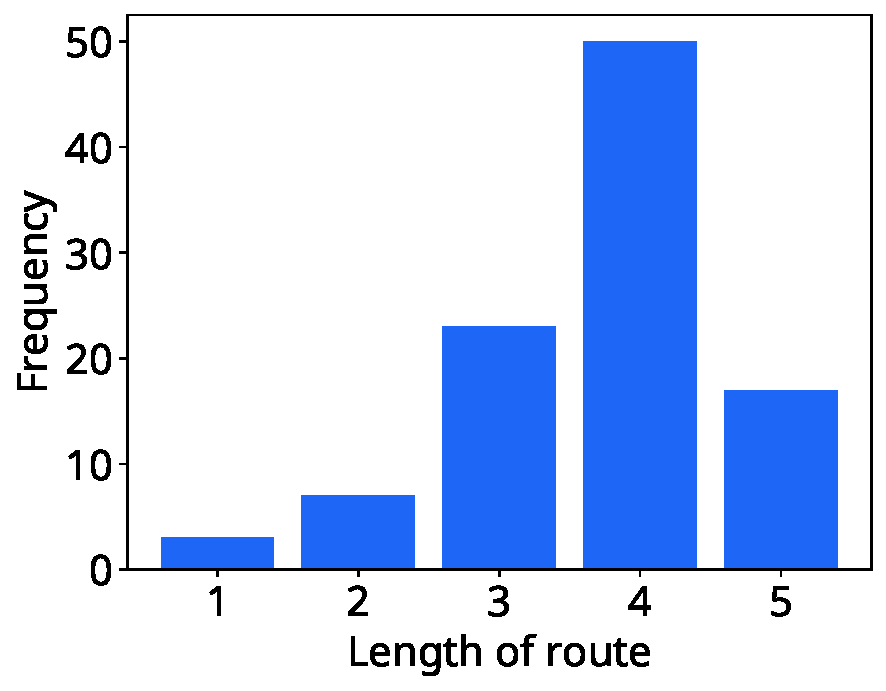
\includegraphics[width=\textwidth]{pictures/plots/topology/route_freq_small.pdf}
% 	\caption{Small}
% 	\end{subfigure}
% 	\begin{subfigure}{0.49\textwidth}
% 	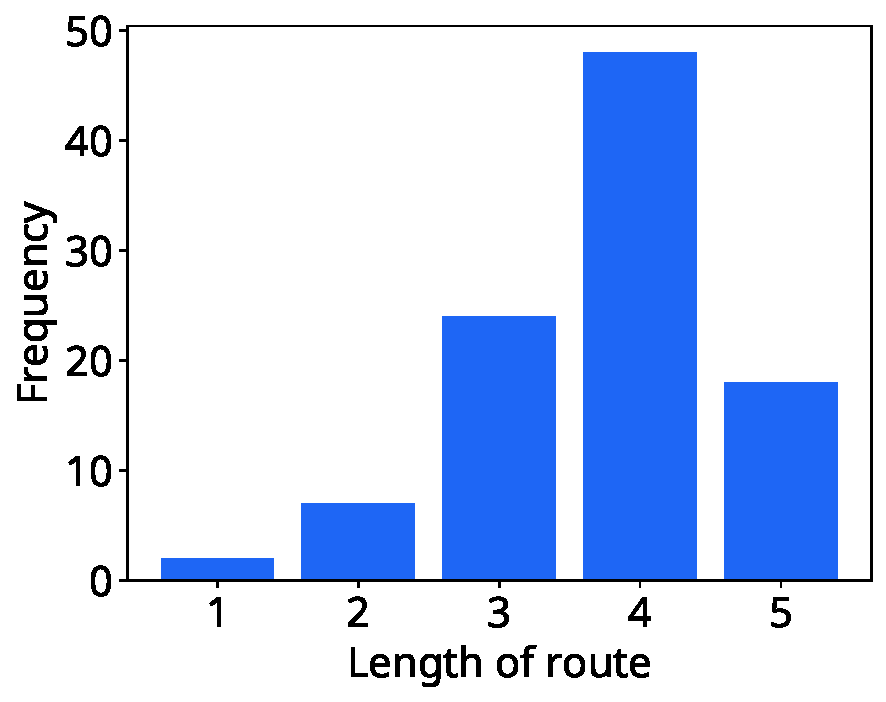
\includegraphics[width=\textwidth]{pictures/plots/topology/route_freq_large.pdf}
% 	\caption{Large}
% 	\end{subfigure}
% 	\caption{The frequency of the length of route (number of links) in each network topology}
% 	\label{fig:toynetworksroutefreq}
% \end{figure}
